\item A particle of mass \( m \) moves along a circle of radius \( R \). Find the modulus of the average vector of the force acting on the particle over the distance equal to a quarter of the circle, if the particle moves
    \begin{enumerate}
        \item uniformly with velocity \( v \);
        \item with constant tangential acceleration \( w_{\tau} \), the initial velocity being equal to zero.
    \end{enumerate}
    \begin{center}
        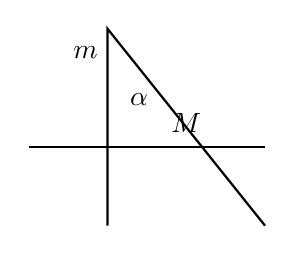
\begin{tikzpicture}
            \draw [thick] (-1,0) -- (2,0);
            \draw [thick] (0,-1) -- (0,1.5) -- (2,-1);
            \node at (1,0.3) {\( M \)};
            \node at (0,1) [above left] {\( m \)};
            \node at (0.4,0.6) {\( \alpha \)};
        \end{tikzpicture}
    \end{center}